%%%%%%%%%%%%%%%%%%%%%%%%%%%%%%%%%%%%%%%%%
% Beamer Presentation
% LaTeX Template
% Version 1.0 (10/11/12)
%
% This template has been downloaded from:
% http://www.LaTeXTemplates.com
%
% License:
% CC BY-NC-SA 3.0 (http://creativecommons.org/licenses/by-nc-sa/3.0/)
%
%%%%%%%%%%%%%%%%%%%%%%%%%%%%%%%%%%%%%%%%%

%----------------------------------------------------------------------------------------
%	PACKAGES AND THEMES
%----------------------------------------------------------------------------------------

\documentclass{beamer}
\usepackage[utf8]{inputenc}
\usepackage{amsmath}
\usepackage{bm}
\usepackage{graphicx}
\usepackage{caption}
\usepackage{subcaption}
\captionsetup{compatibility=false}
\mode<presentation> {

% The Beamer class comes with a number of default slide themes
% which change the colors and layouts of slides. Below this is a list
% of all the themes, uncomment each in turn to see what they look like.

%\usetheme{default}
%\usetheme{AnnArbor}
%\usetheme{Antibes}
%\usetheme{Bergen}
%\usetheme{Berkeley}
%\usetheme{Berlin}
%\usetheme{Boadilla}
%\usetheme{CambridgeUS}
%\usetheme{Copenhagen}
%\usetheme{Darmstadt}
%\usetheme{Dresden}
%\usetheme{Frankfurt}
%\usetheme{Goettingen}
%\usetheme{Hannover}
%\usetheme{Ilmenau}
%\usetheme{JuanLesPins}
%\usetheme{Luebeck}
\usetheme{Madrid}
%\usetheme{Malmoe}
%\usetheme{Marburg}
%\usetheme{Montpellier}
%\usetheme{PaloAlto}
%\usetheme{Pittsburgh}
%\usetheme{Rochester}
%\usetheme{Singapore}
%\usetheme{Szeged}
%\usetheme{Warsaw}

% As well as themes, the Beamer class has a number of color themes
% for any slide theme. Uncomment each of these in turn to see how it
% changes the colors of your current slide theme.

%\usecolortheme{albatross}
%\usecolortheme{beaver}
%\usecolortheme{beetle}
%\usecolortheme{crane}
%\usecolortheme{dolphin}
%\usecolortheme{dove}
%\usecolortheme{fly}
\usecolortheme{lily}
%\usecolortheme{orchid}
%\usecolortheme{rose}
%\usecolortheme{seagull}
%\usecolortheme{seahorse}
%\usecolortheme{whale}
%\usecolortheme{wolverine}

%\setbeamertemplate{footline} % To remove the footer line in all slides uncomment this line
%\setbeamertemplate{footline}[page number] % To replace the footer line in all slides with a simple slide count uncomment this line

%\setbeamertemplate{navigation symbols}{} % To remove the navigation symbols from the bottom of all slides uncomment this line
}

\usepackage{graphicx} % Allows including images
\usepackage{booktabs} % Allows the use of \toprule, \midrule and \bottomrule in tables

%----------------------------------------------------------------------------------------
%	TITLE PAGE
%----------------------------------------------------------------------------------------

\beamertemplatenavigationsymbolsempty

\title[Camassa-Holm]{Exploring a finite difference scheme \\ for the Camassa-Holm equation} % The short title appears at the bottom of every slide, the full title is only on the title page

\author{Halvorsen, \O sthus and Longva} % Your name
\institute[NTNU] % Your institution as it will appear on the bottom of every slide, may be shorthand to save space
{
Norwegian University of Science and Technology
\medskip
}
\date{April 1 2014} % Date, can be changed to a custom date

\begin{document}

\begin{frame}
\titlepage % Print the title page as the first slide
\end{frame}

%----------------------------------------------------------------------------------------
%	PRESENTATION SLIDES
%----------------------------------------------------------------------------------------
\section{Presentation of the Camassa-Holm equation}
\begin{frame}
\frametitle{The Camassa-Holm equation}

\begin{align*}
u_{t} - u_{xxt} + 3uu_{x} - 2u_{x}u_{xx} - uu_{xxx} = 0,
\end{align*}


\begin{align*}
m &= u - u_{xx} \notag \\
m_t &= -2mu_x - um_x.
\label{eq:CHhamiltonian}
\end{align*}

Peaked solitons (peakons) are weak solutions:
\begin{align*}
u(x, t) = ce^{-|x - ct|}
\end{align*}

\end{frame}


\section{Single peakon}
\begin{frame}
\frametitle{Single peakon}

\begin{figure}
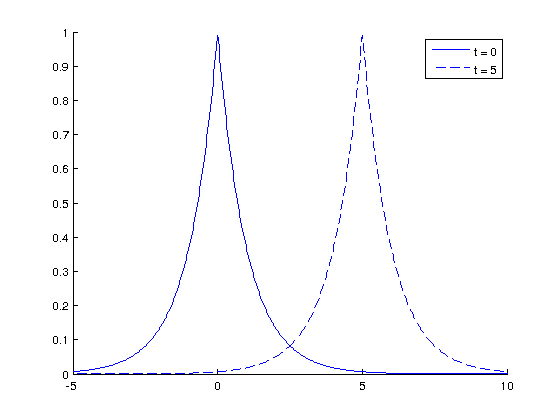
\includegraphics[width=0.8\linewidth]{gfx/peakon}
\end{figure}

\end{frame}


\section{Double peakon}
\begin{frame}
\frametitle{Double peakon}

\begin{figure}
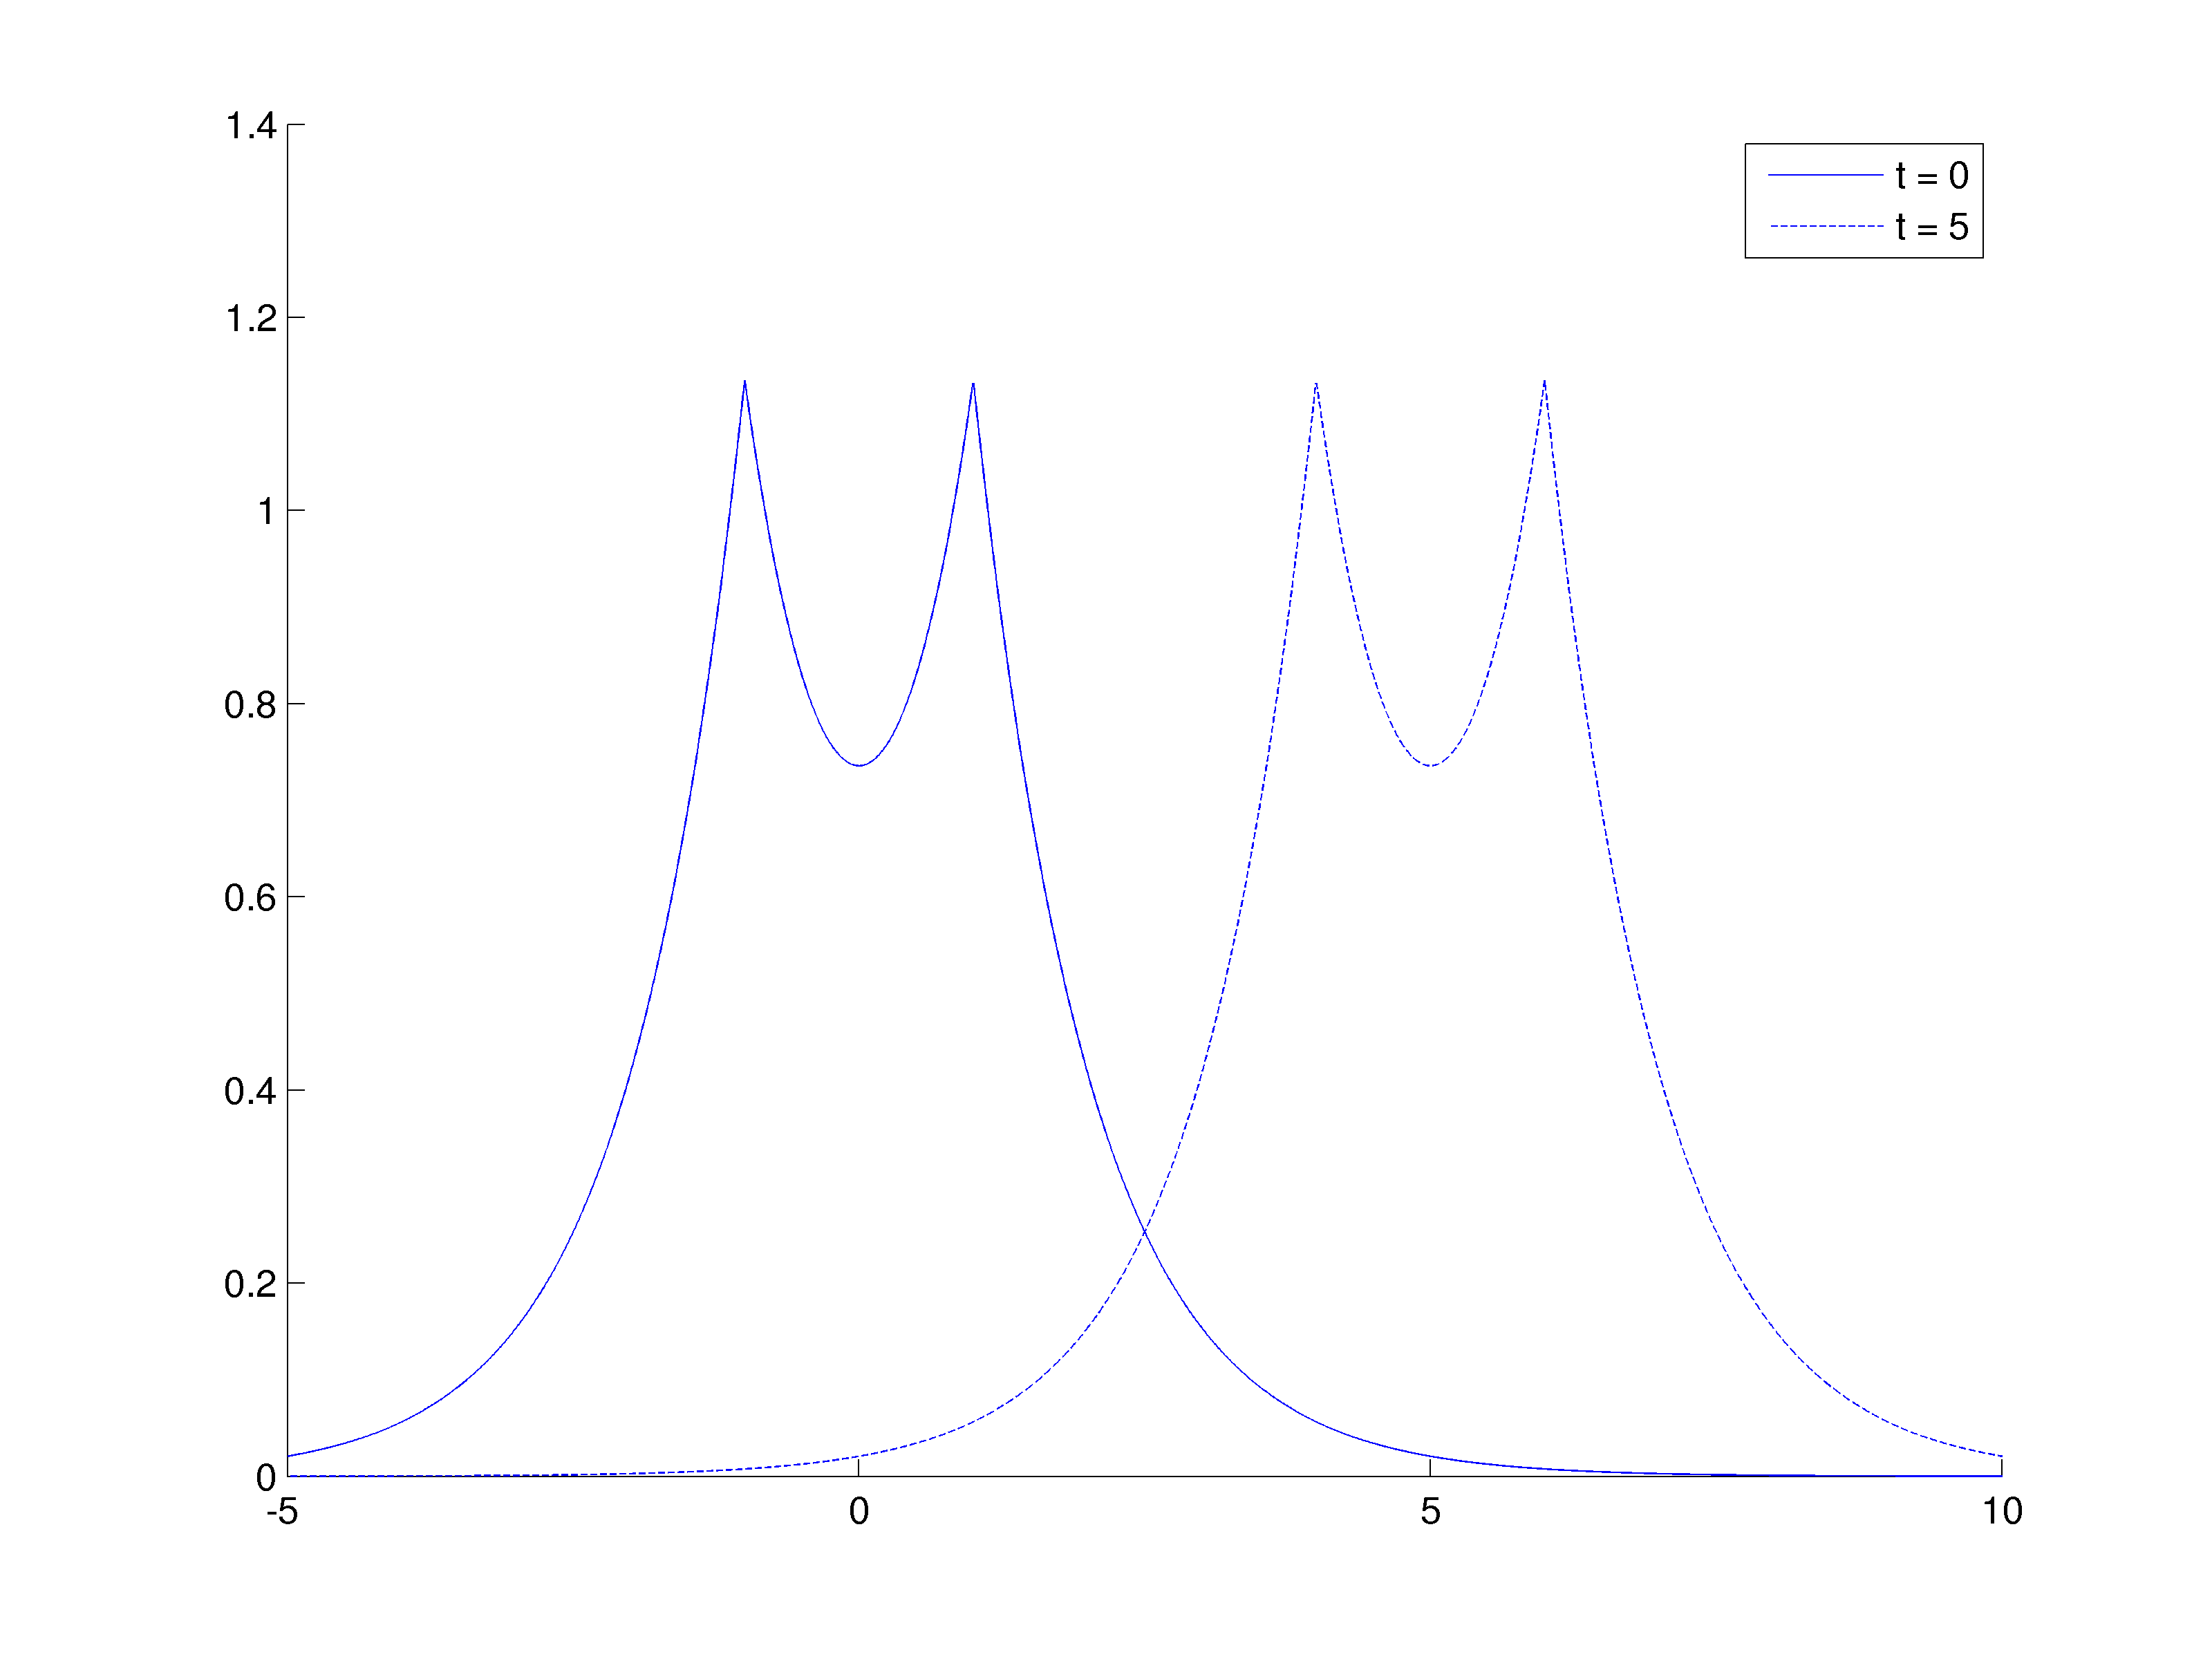
\includegraphics[width=0.8\linewidth]{gfx/doublepeakon}
\end{figure}

\end{frame}


\section{Peakon interaction}
\begin{frame}
\frametitle{Peakon-peakon interaction, different heights}

\begin{figure}
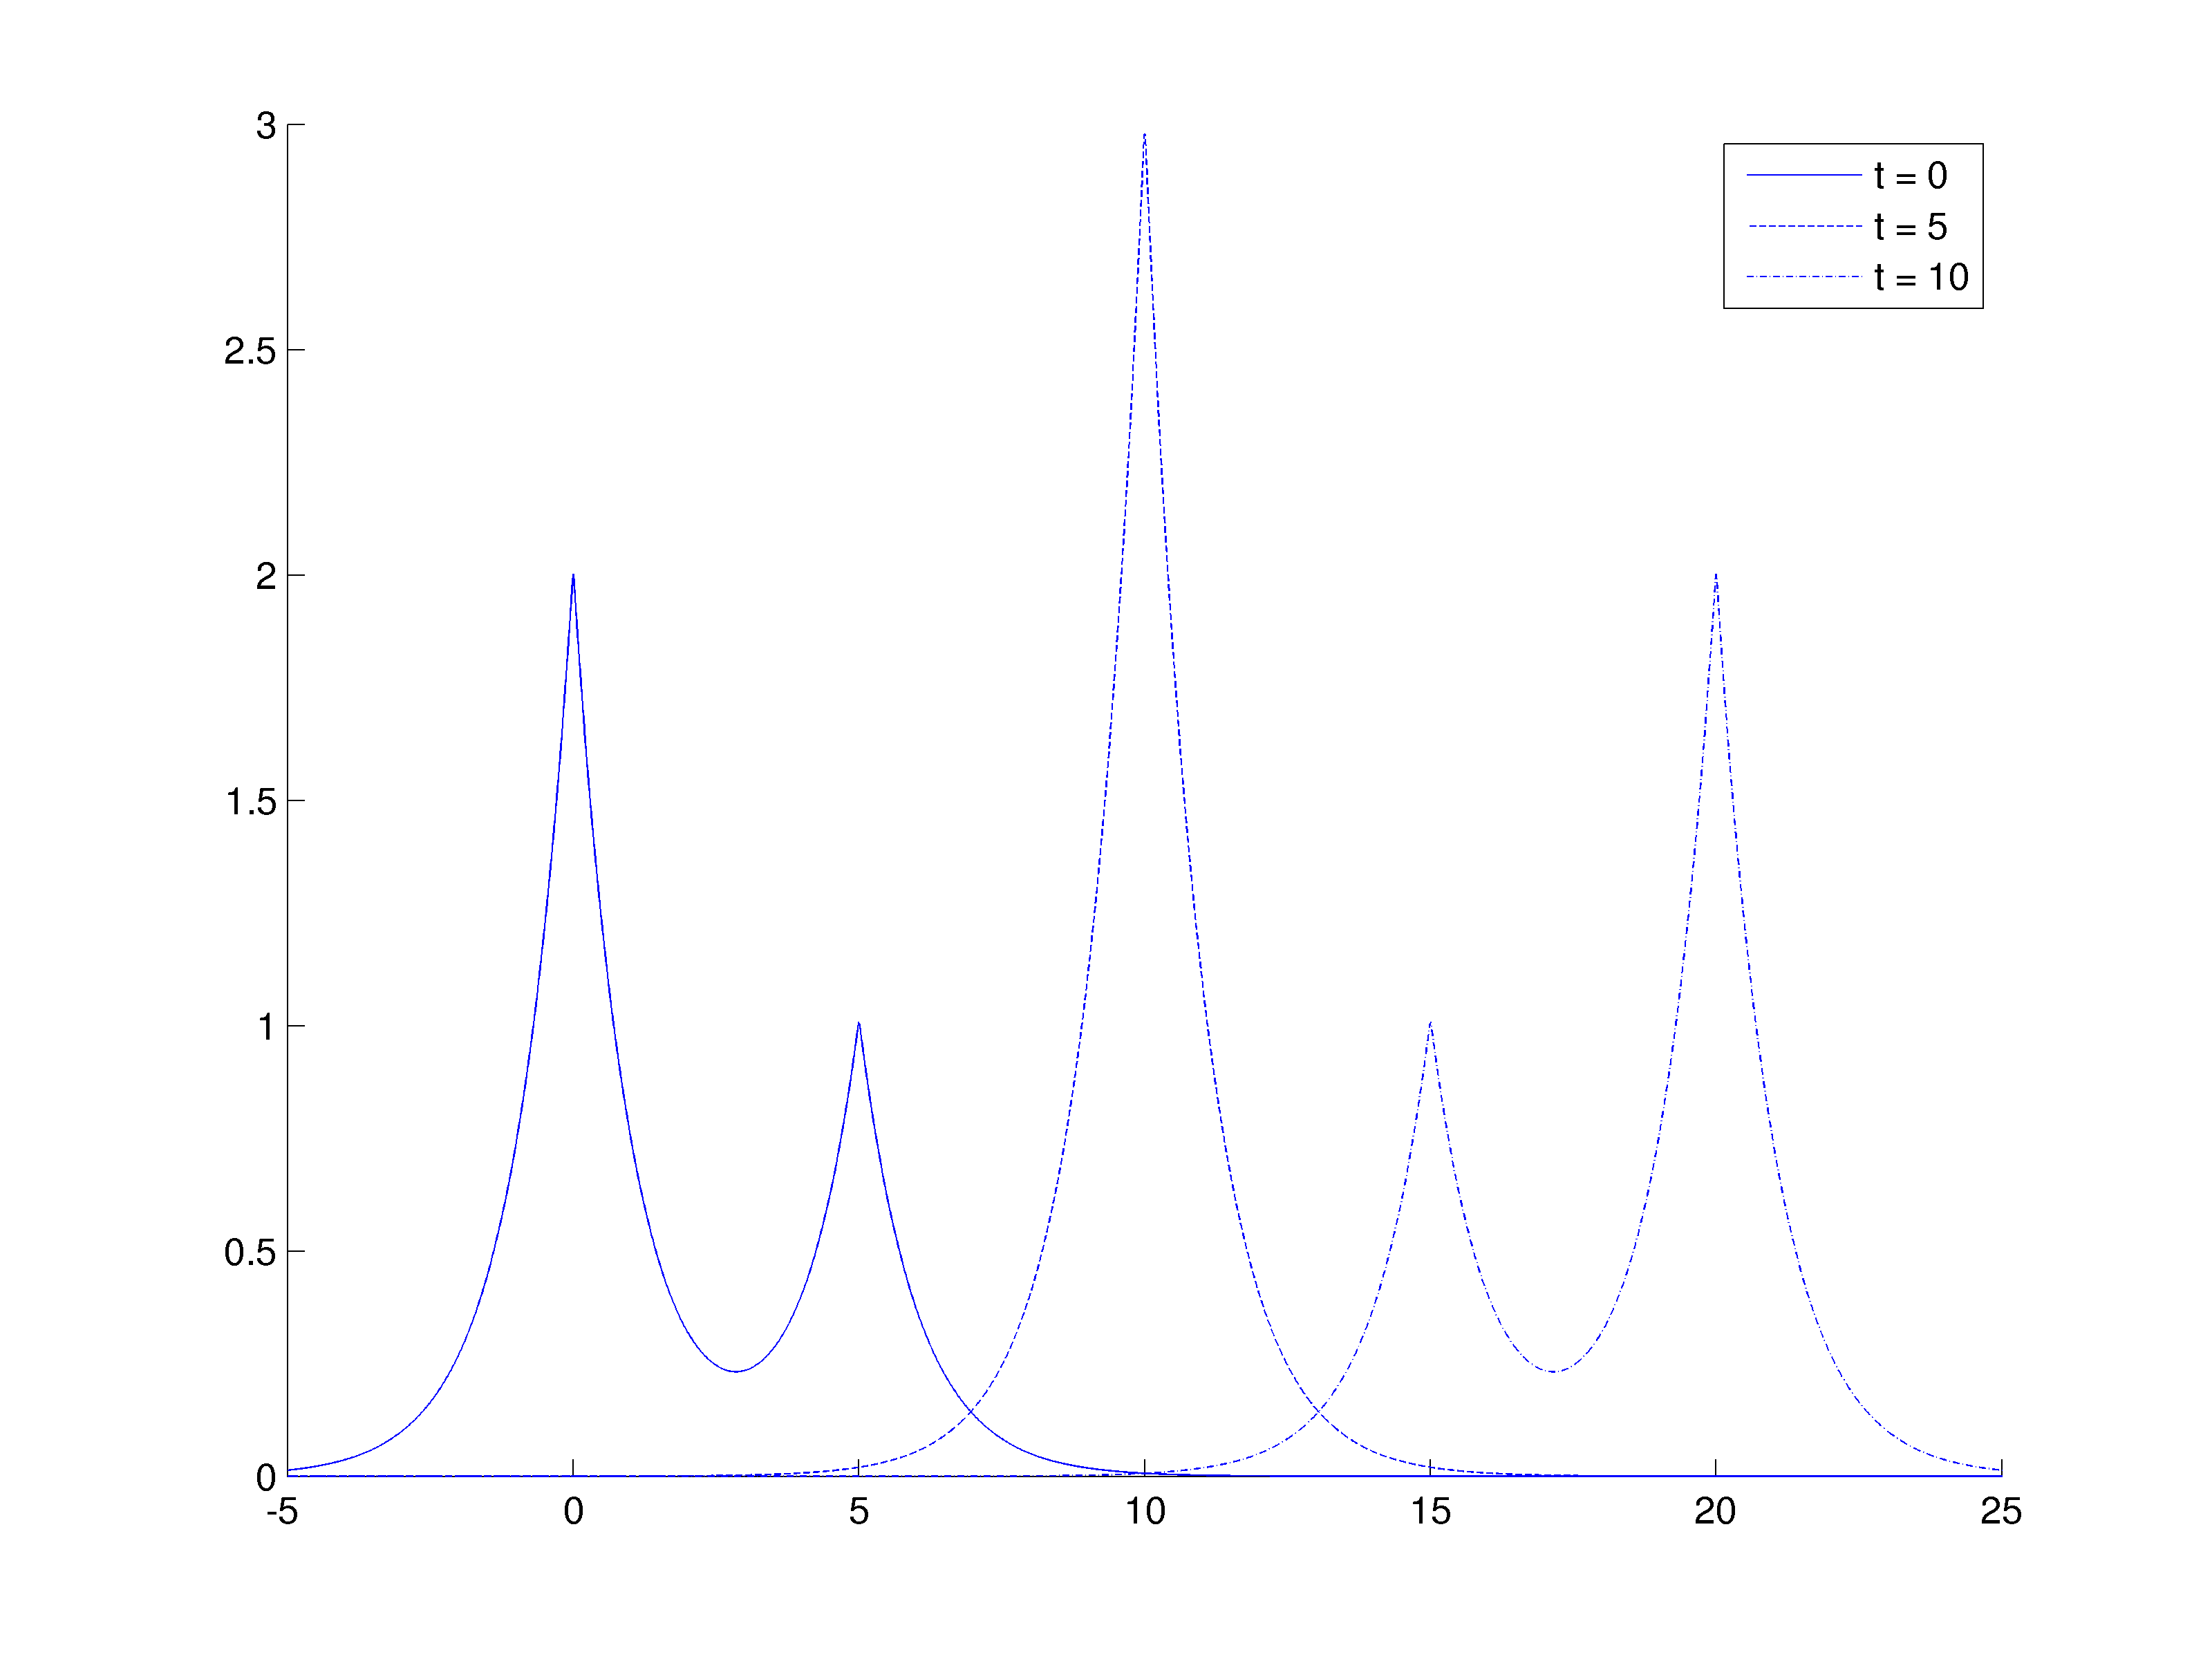
\includegraphics[width=0.8\linewidth]{gfx/peakonovertake}
\end{figure}

\end{frame}


\section{Peakon/antipeakon}
\begin{frame}
\frametitle{Peakon-antipeakon interaction}
\begin{figure}
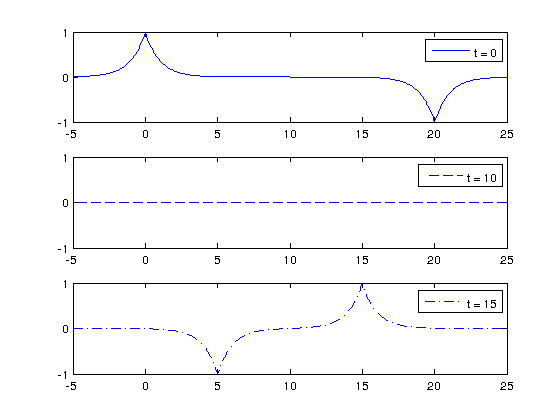
\includegraphics[width=0.8\linewidth]{gfx/peakonantipeakon}
\end{figure}

\end{frame}


\begin{frame}
\frametitle{The finite difference scheme}

\begin{align*}
%m &= Au,\\
m &= u - D_- D_+ u \notag \\
m_t &=- D_- ( m u ) - m D ( u ), 
\end{align*} 

\vspace{3.5cm}

\tiny{H. Holden, X. Raynaud, Convergence of a finite difference scheme for the Camassa-Holm equation}


\end{frame}



\section*{More scheme}
\begin{frame}
\frametitle{Matrix notation}
\begin{align*}
\bm{m}^{n+1} &= \bm{m}^{n} + k \left[- \bm{B} (\bm{M}^n \bm{u}^n) - \bm{M}^n \bm{D} (\bm{u}^n)\right] \\
\bm{Au}^{n + 1} &= \bm{m}^{n+1},
\end{align*}

where 
\begin{align*}
\bm{M}^n = 
\begin{pmatrix}
  m_1^{n} & \cdots & 0 \\
  \vdots  & \ddots & \vdots  \\
  0 & \cdots & m_N^n
 \end{pmatrix}
\end{align*}

\end{frame}




\section*{Extended scheme}
\begin{frame}
\frametitle{Extension of scheme to handle antipeakons}
\begin{align*}
\text{Original} \\
m &= u - D_- D_+ u \notag \\
m_t &=- D_- ( m u ) - m D ( u ), \\ \\
\text{Extended} \\
m &= u - D_{-}D_{+}u, \notag \\ 
m_t &= -D_{-}(m(u \vee 0)) -D_{+}(m(u \wedge 0)) - mD(u), 
\end{align*}

$u \vee 0 = max(u, 0)$ \\
$u \wedge 0 = min(u, 0) $

\vspace{1cm}
\tiny{M. L. Dahlby, Geometric integration of nonlinear
wave equations}
\end{frame}


\section*{CFL condition}
\begin{frame}
\frametitle{Necessary condition for stability}
The CFL condition
\begin{align*}
c \frac{\Delta t}{\Delta x} \leq 1
\end{align*}

\begin{figure}
\begin{subfigure}[b]{0.49\textwidth}
                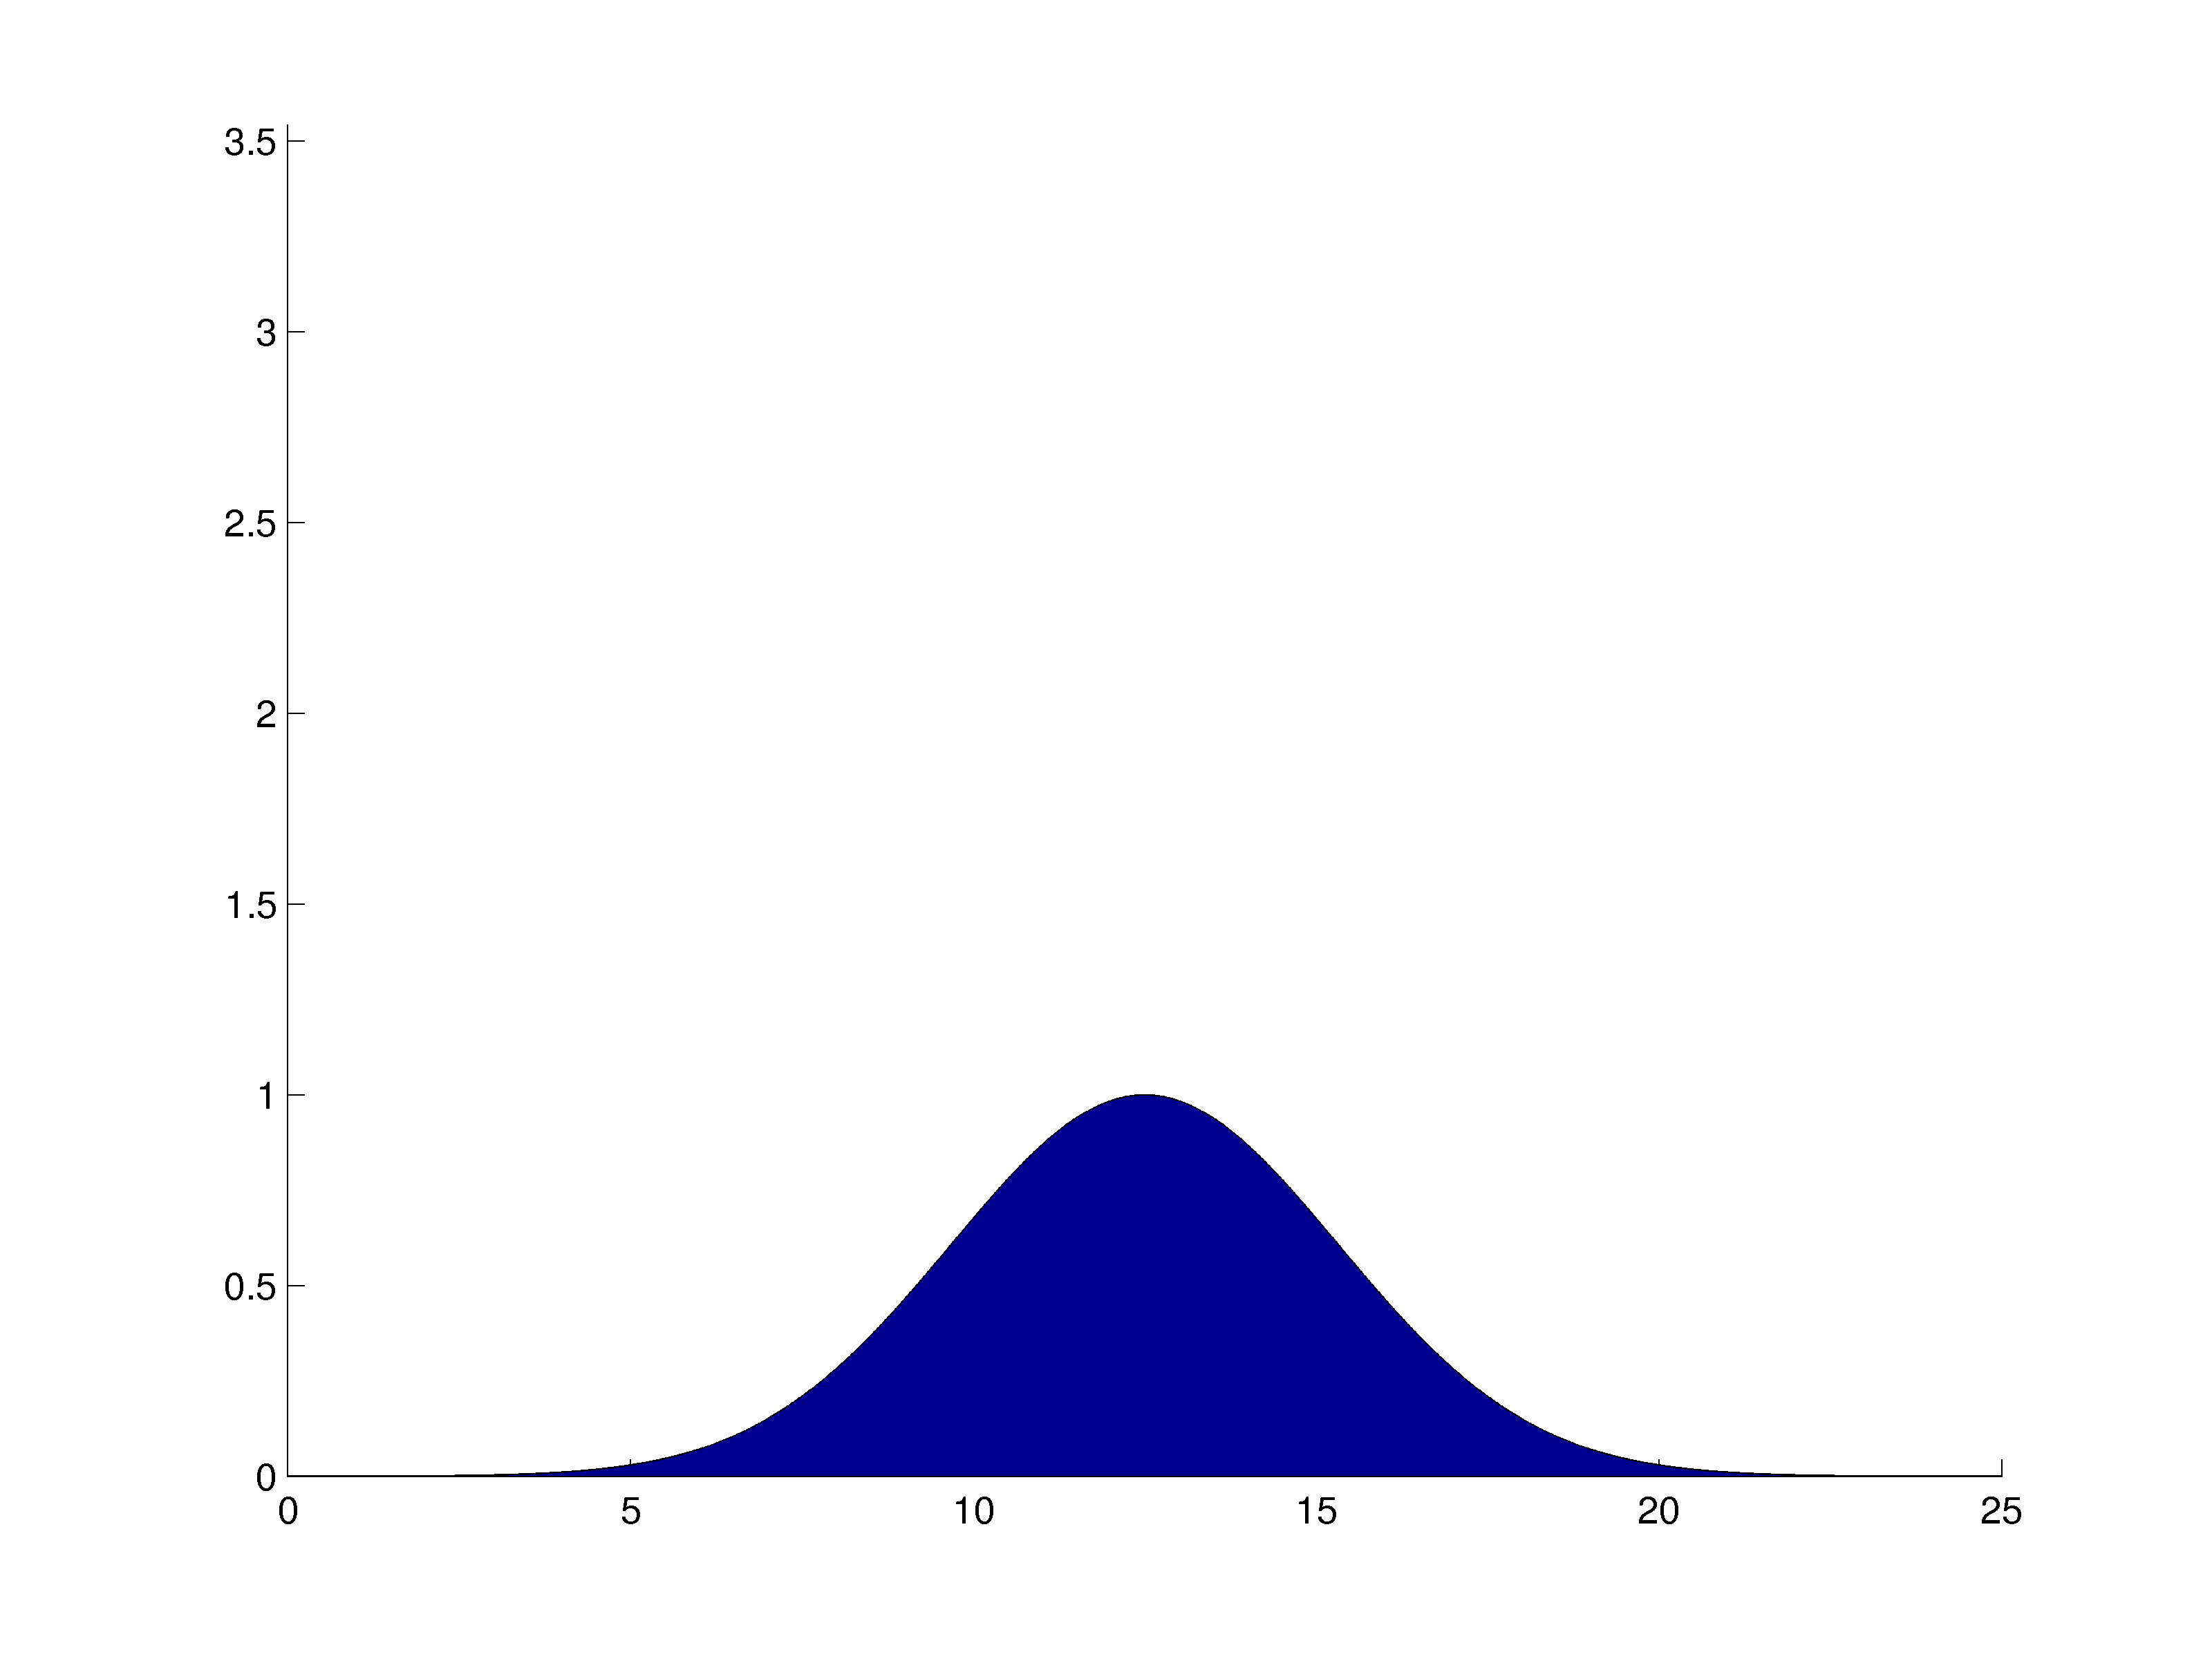
\includegraphics[width=\textwidth]{gfx/areainitial}
\end{subfigure}
\begin{subfigure}[b]{0.49\textwidth}
                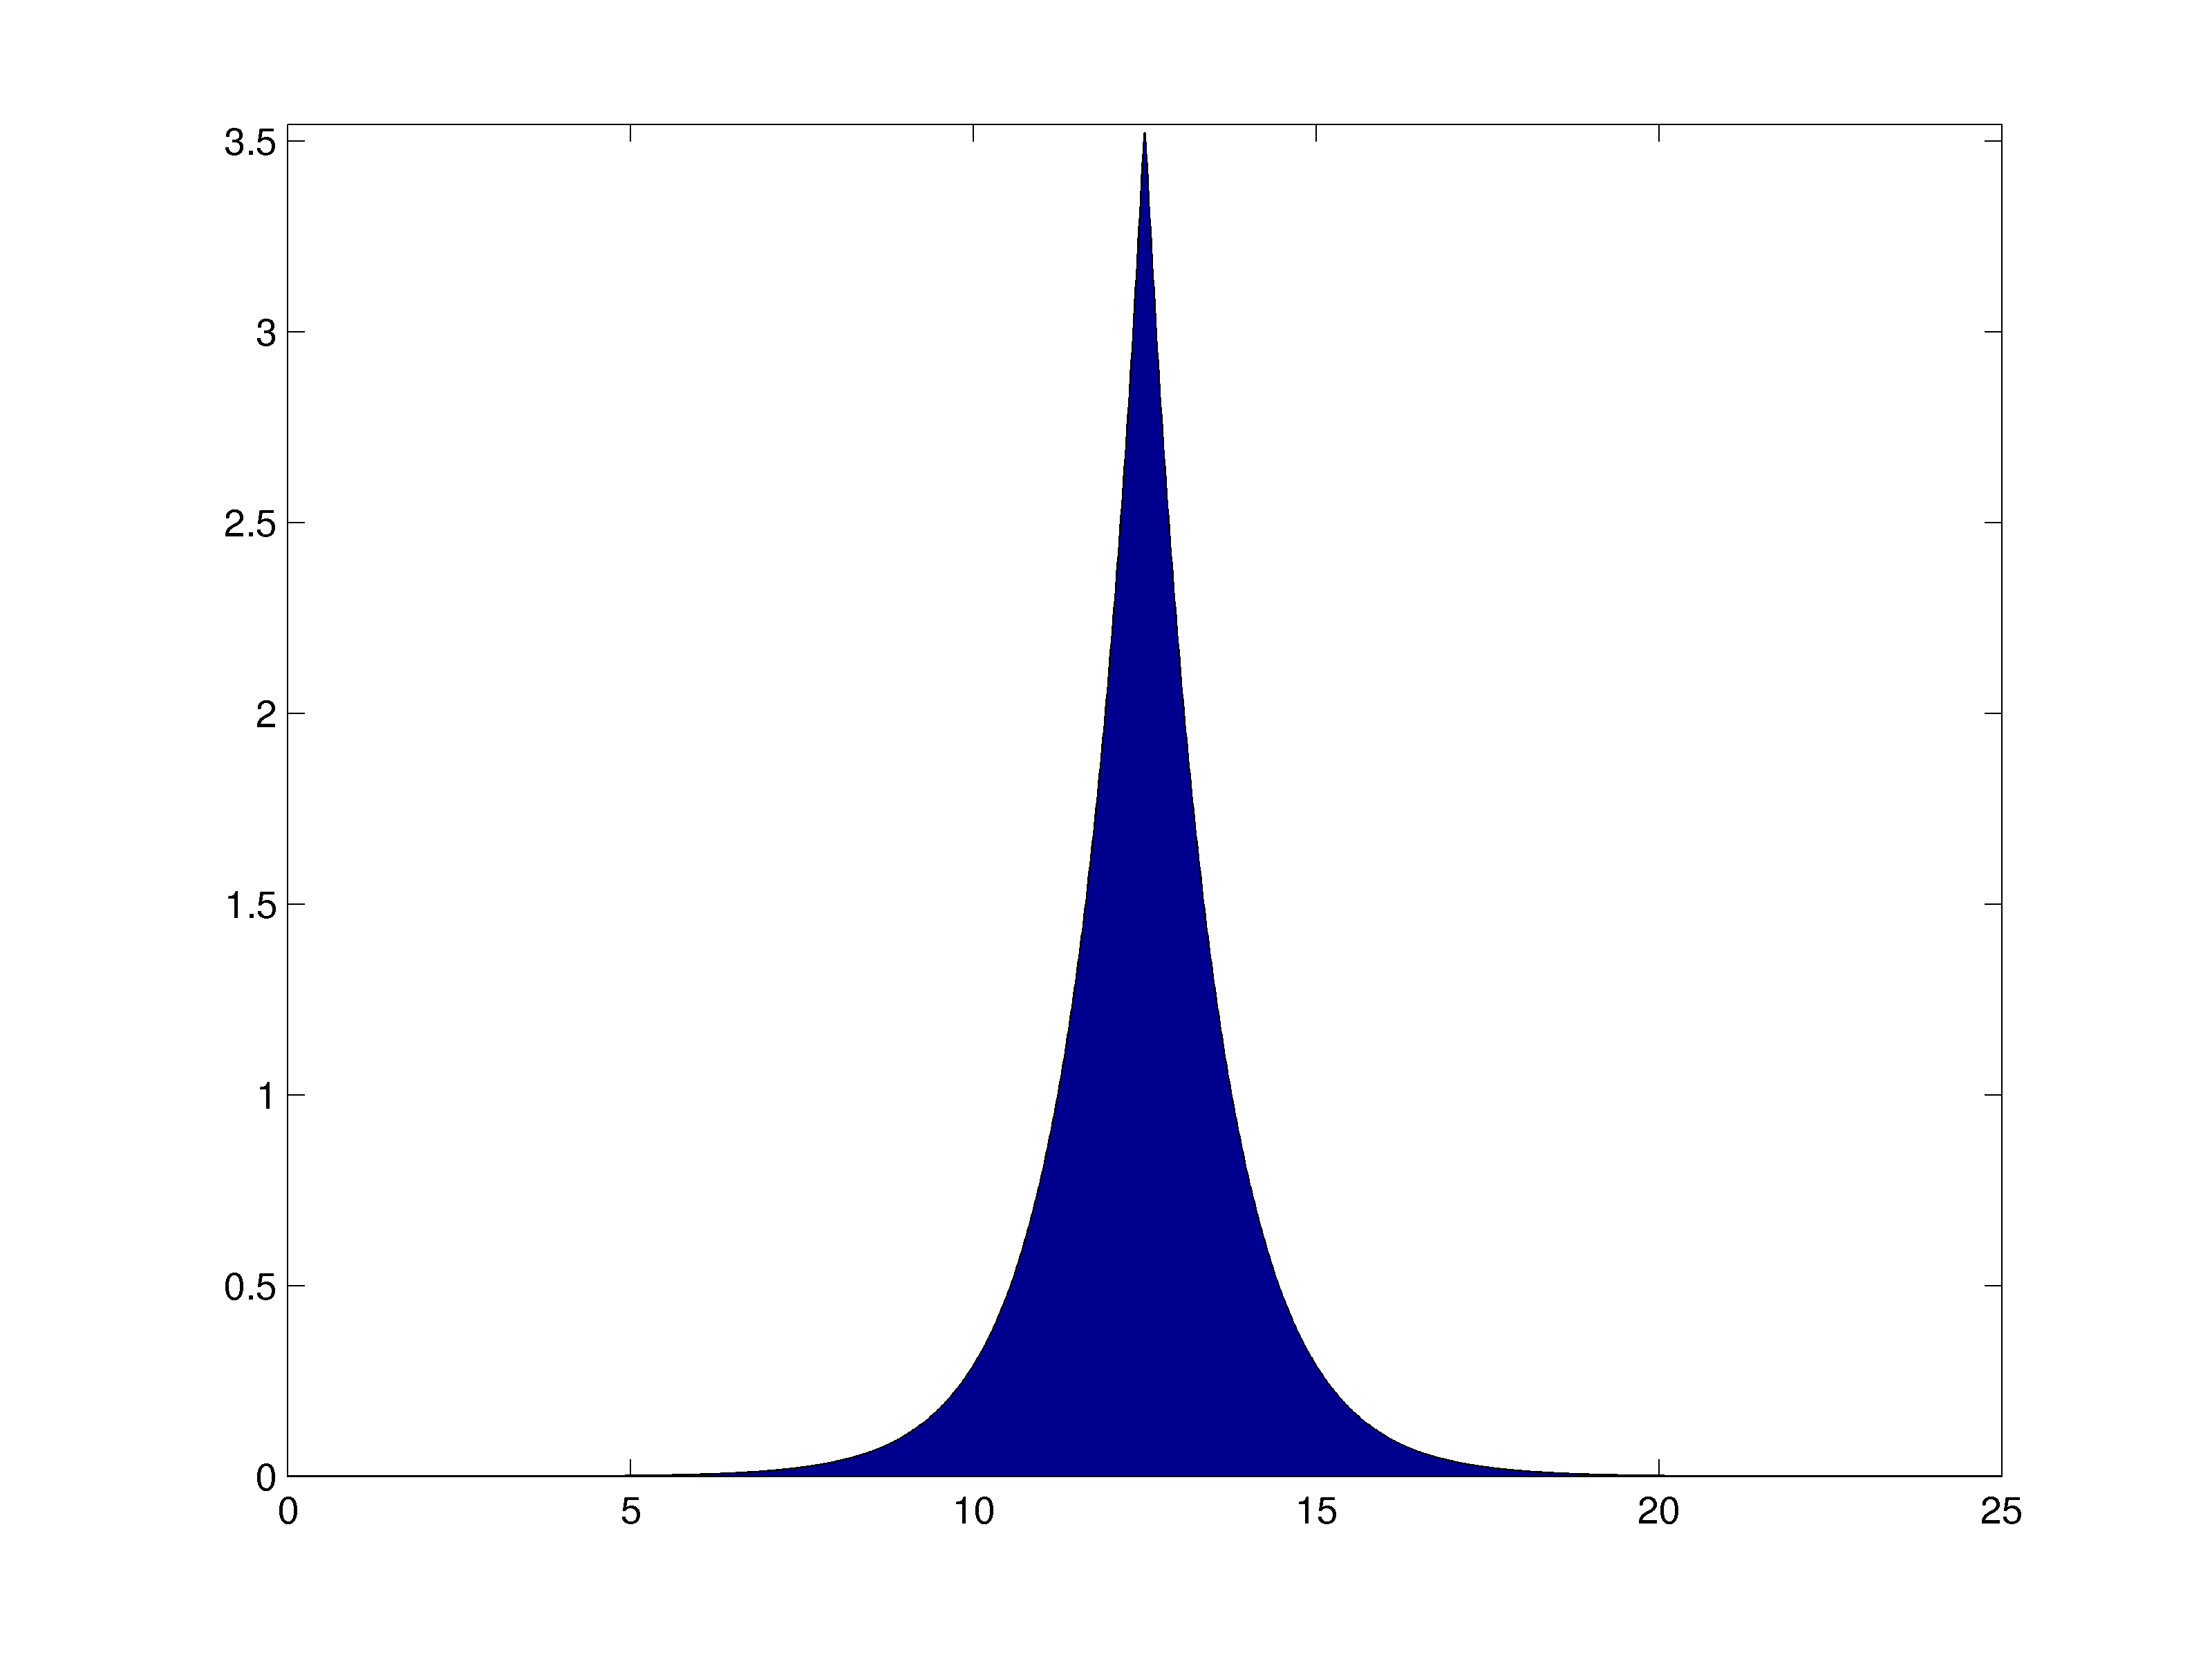
\includegraphics[width=\textwidth]{gfx/areapeakon}
\end{subfigure}
\end{figure}

\end{frame}


\section*{Numerical convergence}
\begin{frame}
\frametitle{Convergence in space}
\begin{figure}
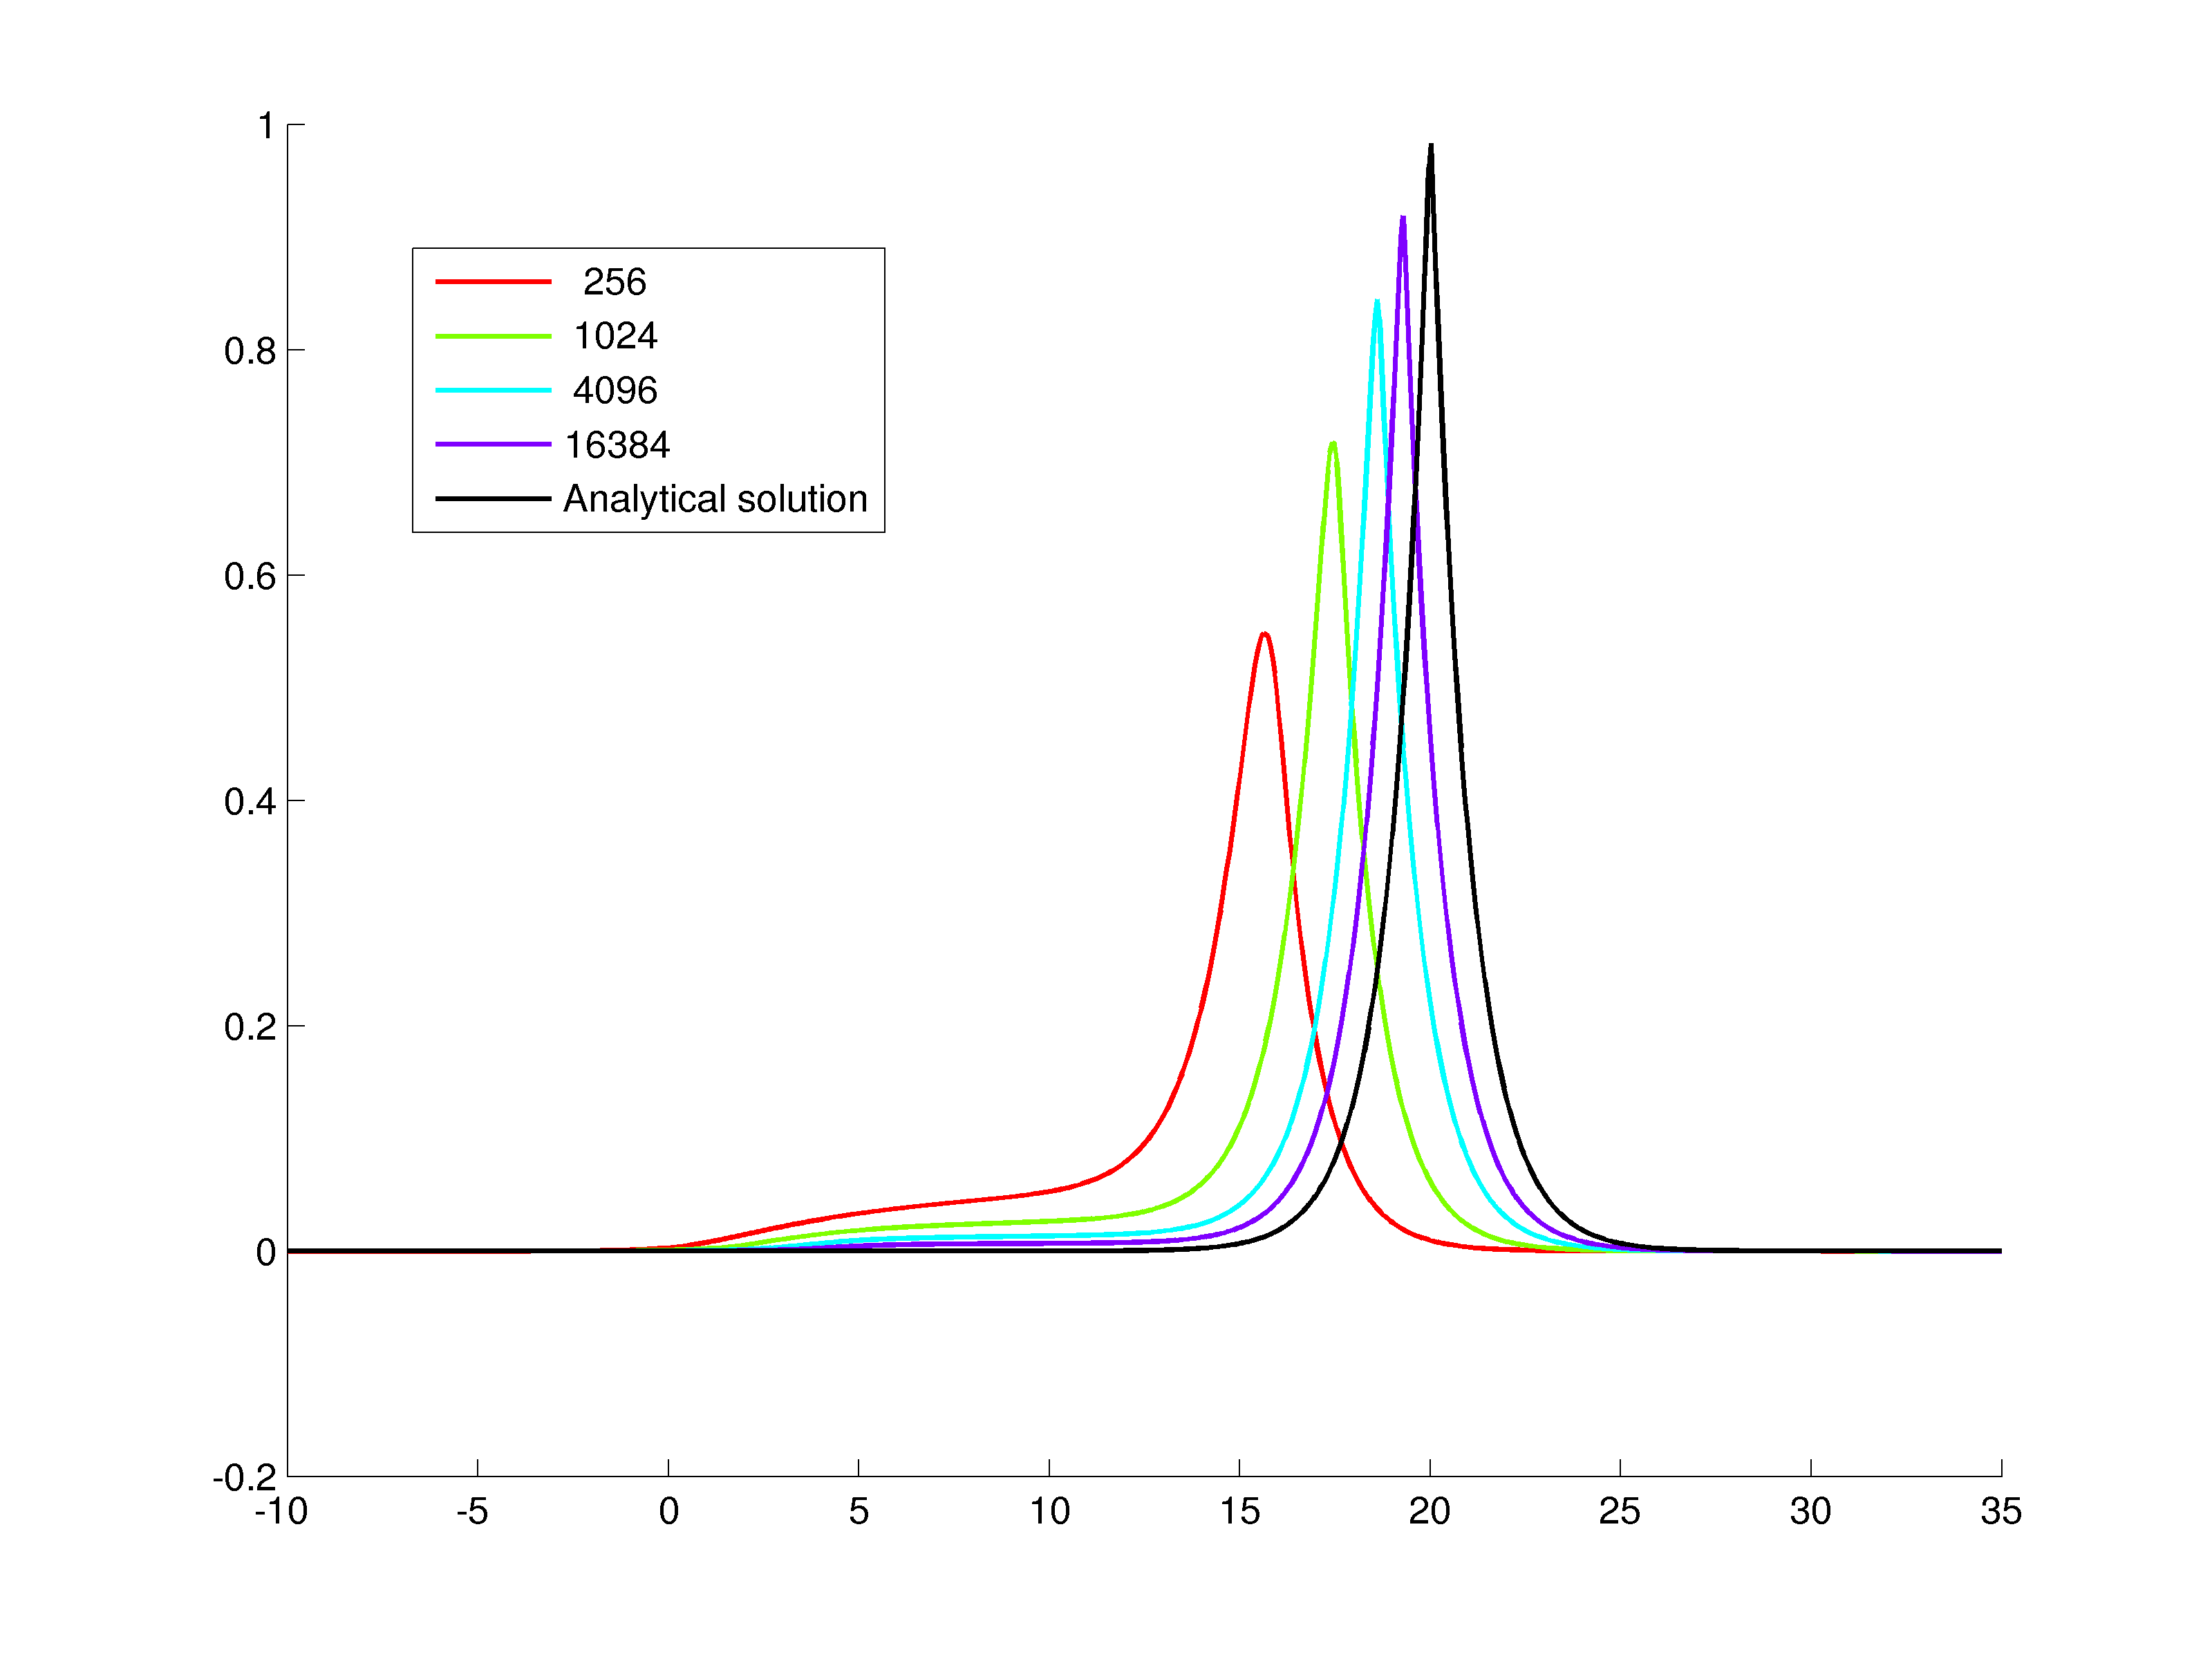
\includegraphics[width=0.8\linewidth]{gfx/attimeT}
\end{figure}
\end{frame}

\section*{Order of convergence}
\begin{frame}
\frametitle{Order of convergence}
\begin{figure}
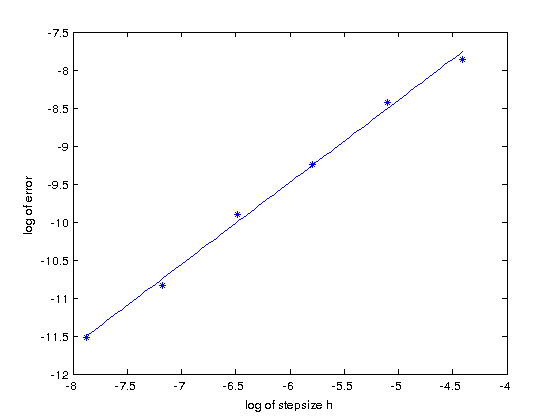
\includegraphics[width=0.8\linewidth]{gfx/loglog}
\end{figure}
\end{frame}

\section*{Analysis}
\begin{frame}
\frametitle{Analysis}
\begin{itemize}
\item Convergence, stability proved by Holden and Raynaud
\item We were able to verify consistency
\item Von Neumann stability analysis offers no conclusion
\end{itemize}
\end{frame}

\section*{Stability}
\begin{frame}
\frametitle{Stability}
\begin{align*}
\bm{m}^n &= (\bm{I}-\bm{BF})\bm{u}^n = \bm{A} \bm{u}^n \\
\bm{m}^n_t &= -\bm{BM}^n \bm{u}^n - \bm{M}^n\bm{Cu}^n = \bm{-Qu}^n,
\end{align*}

\begin{align*}
\bm{m}^{n+1} &= \bm{m}^n + k\bm{m}^n_t \\
\bm{m}^{n+1} &= \bm{m}^n - k\bm{Qu}^n \\
\bm{u}^{n+1} &= \bm{A}^{-1} \bm{m}^{n+1} = \left(\bm{I} -\bm{A}^{-1} k\bm{Q}\right)\bm{u}^n = \bm{Zu}^n.
\end{align*}
\end{frame}

\section*{Implementation}
\begin{frame}
\frametitle{Improving computational efficiency}

\begin{align*}
\bm{Au} = \bm{m}
\end{align*}

Alternative: discrete convolution product
\begin{align*}
u = \mathcal{F}^{-1} (\mathcal{F} (g) \cdot \mathcal{F}(m))
\end{align*}

Result: $77\%$ reduction in computational time

\vspace{2cm}
\tiny{Definition of g presented in paper by Holden and Raynaud}
\end{frame}

\end{document} 